\documentclass{article}

% Language setting
% Replace `english' with e.g. `spanish' to change the document language
\usepackage[english]{babel}

% Set page size and margins
% Replace `letterpaper' with`a4paper' for UK/EU standard size
\usepackage[letterpaper,top=2cm,bottom=2cm,left=3cm,right=3cm,marginparwidth=1.75cm]{geometry}

% Useful packages
\usepackage{amsmath}
\usepackage{graphicx}
\usepackage{natbib}

\usepackage[colorlinks=true, allcolors=blue]{hyperref}

\title{Elliptic Curves and the Nagell-Lutz theorem:\\a guided reinvention}
\author{Samuel Dauncey}

\begin{document}
\maketitle

\begin{abstract}
    
"Number theory has an annoying habit: the field produces, without effort, innumerable problems which have a sweet, innocent air about them, tempting flowers; and yet... number theory swarms with bugs, waiting to bite the tempted flower-lovers who, once bitten, are inspired to excesses of effort!" - Barry Mazur
\end{abstract}

\section{Introduction and Motivation}

\subsection{An innocent-looking problem}

Suppose one wanted to find all solutions to the polynomial equation:

\[3 X^3 +  2 X Y^2 + 2 Y^3 = Z^3 \quad \text{For integers $X$, $Y$ and $Z$}\].

 One may realise that, given a solution; say $(X, Y, Z) = (1, 2, 3)$, one can see that we can generate infintely many more solutions $(X, Y, Z) = (2, 4, 6), \; (3, 6, 9), \; \dots \; (n, 2n, 3n) \; \dots $. This property of our equation is special, it is called \emph{homogeneity} and stems from the fact that if we sum up the powers of $X$, $Y$ and $Z$ in each of the terms of our equation, we get the same integer (in this case, three). \\
 
 Finding solutions to homogeneous equations is of special importance to number theorists, examples including the Fermat equations $X^m + Y^m = Z^m$. \\
 
 In essence, we can think of each of these infinite sets of solutions as all part of the same solution, and we can see that, if we view our solutions as coordinates in $R^3$, each one of our infinite sets of solutions can be viewed as a line going through the origin and and a point with integer coordinates. Dividing our original equation by $Z$, we can see that our problem is equivalent to finding the rational solutions to the equation:
 
 \[3x^3 + 2xy^2 + 2y^3 = 1\]
 
With rational solution $(x, y) = (\frac{m}{n}, \frac{p}{q})$ being converted into $(X, Y, Z) = (m, p, nq)$ and integer solution $(X, Y, Z)$ being converted into $(\frac{X}{Z}, \frac{Y}{Z})$. However, note that this conversion isn't well-defined when $Z = 0$, so we still have to consider the integer solutions to $3 X^3 +  2 X Y^2 + 2 Y^3 = 0$. However; as this is also a homogeneous polynomial equation, we can repeat our process, this time by dividing by $Y$ to see we want to find solutions to: 

\[3 x^3 + 2 x + 2 = 0 \quad \text{for rational $x$ and $X^3 = 0$ for integer $X$}\]

Hence, we can see that there is a one-to-one correspondence between the "lines" of integer solutions to $3 X^3 +  2 X Y^2 + 2 Y^3 = Z^3$ and rational solutions to  $3x^3 + 2xy + y^3 = 1$, \quad $3 x^3 + 2 x + 2 = 0$, and $X^3 = 0$. Thinking back to our visualisation of our solutions to our integer equation as lines, we can see that our first division resembles looking at the intersection of the plane $Z = 1$ and our solution lines, and the fact that we could recursively apply this procedure is a hint that the \emph{projective space} we are working in has some kind of recursive structure.

Now, we can trivially solve $X^3 = 0 $ to see that $X = 0$ is the only solution (corresponding to the solution $(X, Y, Z) = (0, 0, 0)$). Slightly more difficult is the rational solutions to $3x^3 + 2 x + 2 = 0$; Gauss's Lemma tells us that any solution in it's lowest terms $x = \frac{m}{n}$ must have $m$ dividing $2$ and $n$ dividing $3$, however we can see that the only candidates this leaves, $x = +-\frac{2}{3}$ do not solve the equation; so we have no solutions of the form $(X, Y, 0)$ with non-zero $Y$. Hence, we can see that the only thing stopping us from solving our starting problem is finding all the rational solutions to  $3x^3 + 2xy + y^3 = 1$; unfortunately, this turns out to be alot harder. \\

These solutions form an \emph{algebraic curve} when visualised in the $x,y-$plane, and through analysing this curve geometrically we will be able to get some description of our solution.\\

Note that, given two points $(x_1, y_1)$ and $(x_2, y_2)$ on a degree-3 algebraic curve defined by $f(x, y) = 0$, we can find a third point $(x_3, y_3)$ on the curve by projecting a line $\alpha x + \beta y + \gamma = 0$ through them and looking at the intersection with the curve (in general*). On top of this, when we solve these simultaneous equations by eliminating one variable we get two cubics for the $x$ and $y$ coordinates, $a_3 x^3 + a_2 x^2 + a_1 x + a_0 = 0$ , \quad $b_3 y^3 + b_2 y^2 + b_1 y + b_0 = 0$. We know that the sums $x_1 + x_2 + x_3 = -\frac{a_2}{a_3}$ and $y_1 + y_2 + y_3 = -\frac{b_2}{b_3}$ are satisfied; so if $x_1$, $x_2$ and our coefficients are in some field $F$, $x_3$ must also be in $F$; and likewise for our $y$ coordinates, this means that, given a pair of rational solutions we can get another rational solution by projecting a line.

* the case where $a_3$ or $b_3$ are zero corresponds to the case where our line meets our curve asymptotically, or "at infinity", and we will see more about this when we go into projective geometry.\\ 

The first theorem I will explain is Mordell's theorem, which tells us that we can take a finite set of rational points on our curve and, by projecting lines through them, can get every other rational point on our curve.\\

If we now imagine our points $(x_1, y_1)$ and $(x_2, y_2)$ slowly getting closer and closer to each other on our curve, we may also notice that we could just take one point, draw the tangent from it, and get another rational point. For example,\\ 

Take $\left( \frac{1}{3}, \  \frac{2}{3}\right)$, the point corresponding to the initial solution we found. Then, by projecting the tangent line through our curve and seeing where it intersects, we see that we can get a new rational point, namely: $\left( - \frac{3299}{5943}, \  \frac{6767}{5943}\right)$\\

\begin{figure}
\centering
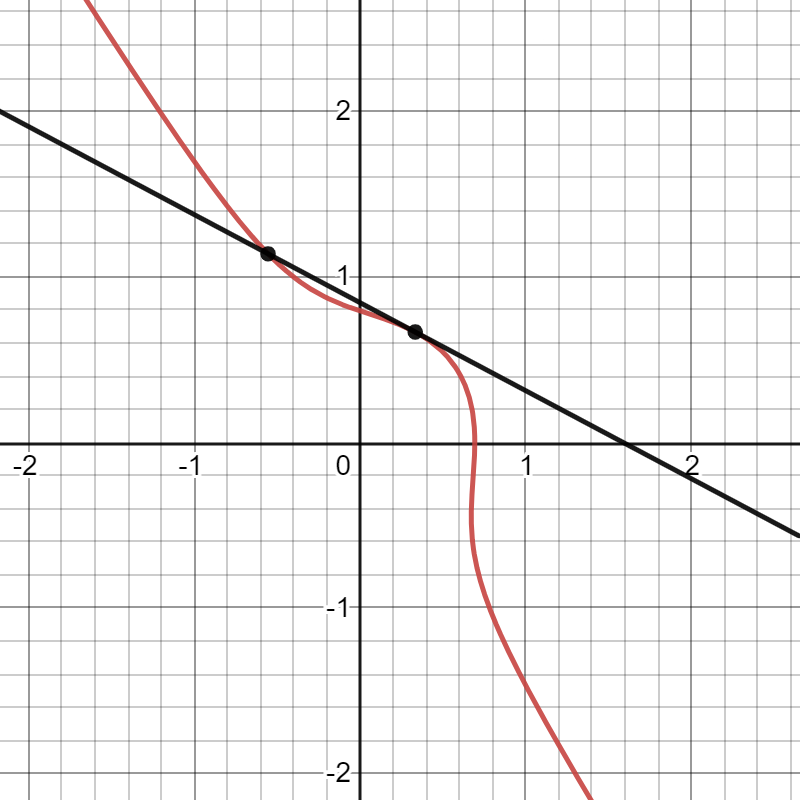
\includegraphics[width=0.5\textwidth]{desmos-graph.png}
\caption{\label{fig:into curve} The tangent of the point $\left( \frac{1}{3}, \  \frac{2}{3}\right)$ on the curve $3x^3 + 2xy^2 + 2y^3 = 1$.}
\end{figure}

The second theorem we will prove is the Nagell-Lutz theorem, which tells us how to find the points will eventually "loop" if we continually apply this process of taking a tangent and seeing where it intersects the curve. After looking deeper into the theory of cubic curves, we will see why these looping points are of particular interest.

\subsection{Assumed prior knowledge}

This report is written to be accessible to first or second-year undergraduates, however the main part of theory that will be assumed knowledge will be familiarity with the concepts of groups, rings and fields. It will follow and use many of the same styles of proofs as \cite{silverman}, however will try and shine a different light on these proofs and fill in some of the parts missed. I made the plots using \cite{desmos} and used my python code for calculations which can be found at \cite{github}.


\newpage

\section{Projective geometry}

\subsection{Homogeneous Coordinates}

In the introduction section, I hinted at the idea that we can think of linearly related solutions, such as $(1, 2, 3)$ and $(2, 4, 6)$ to our homogeneous equation  as one line in $R^3$. We will see that this notion can be made rigorous by defining a new kind of space. We kind of already did this when we divided by $Z$, but this feels unnatural because it is breaking the symmetry of our equation between $X$, $Y$ and $Z$. We will see later that this kind of space is called \emph{projective space} and when we do geometry on this space it is called \emph{projective geometry}, hence the name of this section.\\

We want to define a \emph{point} in projective such that all the solutions $(t, 2t, 3t)$ are considered to be the same object, which is precisely what happened when we divided through by $Z$ in our introduction. So it makes sense to say a point in projective space as a ratio between the $X$, $Y$ and $Z$ coordinates, :\\

We denote $P = [X : Y : Z] \in P_R^2$ for real numbers $X$, $Y$ and $Z$ which are called the \emph{homogeneous} coordinates of $P$;\\

where two points are said to be equal, ie $[X : Y : Z] = [X' : Y' : Z']$ if and only if we can find a $t \in R$ satisfying $X = tX', Y =  tY'$ and $Z = tZ'$\\

Unfortunately, this on it's own is not a well-defined equivalence relation; every point is equal to $[0 : 0 : 0]$. To fix this, we simply ban this point and say if  $[X : Y : Z] \in P_R^2$  then at least one of $X$, $Y$ and $Z$ is non-zero. It is relatively straightforward to now mentally check that this definition of equality satisfies reflexivity, symmetry and transitivity.\\

Note that, if you view the homogeneous coordinates $X$, $Y$ and $Z$ as a point $(X, Y, Z)$ in $R^3$ then our \emph{points} in $P_R^2$ (the equivalence classes of coordinates which give equal points) can be visualised as \emph{lines} going through the origin in $R^3$. Hence, it makes intuitive sense that our \emph{lines} in $P_R^2$ could be visualised as \emph{planes} containing the origin in $R^3$. This intuition gives us the definition of a line in $P_R^2$:\\

A line in $P_R^2$ is the set of points $[X : Y : Z]$ where $AX + BY + CZ = 0$ for some fixed $A$, $B$ and $C$. \\

Note our definition of a line is well defined as  $AX + BY + CZ = 0$ iff  $A(tX) + B(tY) + C(tZ) = 0$ for non-zero $t$. This geometrical intuition gives us an interesting property of lines in $P_R^2$: \\

Two distinct lines in $P_R^2$ intersect at exactly one point. For example, say we have two lines $AX + BY + CZ = 0$ and $\Bar{A}X + \bar{B}Y + \bar{C}Z = 0$. We can solve these equations simultaneously by putting them in a matrix-vector product:\\

$$ \begin{bmatrix}
A & B & C \\
\Bar{A} & \Bar{B} & \Bar{C} 
\end{bmatrix} 
\begin{bmatrix}
X \\
Y \\
Z \\
\end{bmatrix} 
= \vec{0}
$$

From this we can see that, if the two lines are distinct, then $A  B  C$ and
$\Bar{A}  \Bar{B}  \Bar{C} $ will be linearly independent, as if they weren't, we would be able to reduce their defining equations onto each other. Hence our matrix will have rank 2 and so by the rank-nullity theorem we will have one linearly independent solution for $X$, $Y$ and $Z$, corresponding to our point of intersection in $P_R^2$. This property of lines in $P_R^2$ is different to, say, $R^2$, where parallel lines intersect nowhere.\\

When we divided by $Z$ in our introduction, we took each point in $P_R^2$ and mapped it to a point in $R^2$, barring the points where the $Z$ coordinate was $0$. The obvious way to map points in $P_R^2$ onto a surface is to look at projecting them onto the upper half of the unit sphere, using the angles as coordinates. For example mapping $[1 : 2 : 3]$ to the point $(arctan(\frac{1}{2}), arccos(\frac{3}{\sqrt{5}}))$. The problem with this approach is that this takes a point with rational coordinates and maps it to angles without rational coordinates; meaning it isn't very useful for us. Instead, we have to suffice by projecting our projective plane onto a flat screen.\\

Specifically, for each line that goes through the origin in $R^3$, we can look at where this line intersects the plane $Z = 1$; unless the line happens to be parallel to this plane. This is one way of visualising the mapping that takes each point $P_R^2$ with non-zero $Z$ and maps it to a point in the euclidean plane $R^2$ taking $[X : Y : Z] \mapsto (\frac{X}{Z}, \frac{Y}{Z})$. Now let us examine the structure of the points where the $Z$ coordinate is $0$. We see that the set of ratios $[X : Y : 0]$ is very like the projective plane, just with one less dimension. In fact, this structure is called the \emph{projective line}, denoted $P_R^1$ and when view it as a "line at infinity" outside of $R^2$ where the $Z$ coordinate $0$ points get mapped to when we project $P_R^2$ onto $Z = 1$. Thinking about this more generally gives the n-dimensional case, which we won't use but is good to know for intuition:

\[P_R^n \cong A^n \cup P_R^{n-1}\]

 Note that in this section I used the real numbers, $R$ as the field that we were working over. However, the proofs used no special properties about the real numbers, hence we could replace $R$ with any field $F$ and get the same results. In general, we call $P_F^2$ the \emph{projective plane over the field} $F$,  alot of algebraic geometry is concerned with $P_C^2$ for instance, however for us it suffices to know that $P_Q^2$ is well defined.

\subsection{Projective Transformations}

Note that our decision to project onto the plane $Z = 1$ was completely arbitrary. We could have instead projected onto the plane $Y = 2$, mapping the point $[X : Y : Z]$ to $(\frac{2X}{Y}, \frac{2Z}{Y})$ and taking care of points with 0 $Y$ coordinate. In general, we can identify a screen that we want to project onto with three vectors: $\vec{v_x}, \vec{v_y}, \vec{c}$. If we want to project a point $[X : Y : Z]$ onto $(x, y) \in R^2$ through the screen defined by these vectors, we find the unique $x$ and $y$ values such that 

\[\vec{c} + x \vec{v_x} + y \vec{v_y}\]

Is in the line through the origin in $R^3$ which contains $(X, Y, Z)$. Equivalently, we want: 

\[[X : Y : Z] = [c_1 + x (v_x)_1 + y (v_y)_1  \ : \ c_2 + x (v_x)_2 + y (v_y)_2 \ : \ c_3 + x (v_x)_3 + y (v_y)_3]\]

In fact, we can combine these three vectors into a matrix: $M = (v_x | v_y | c)$. Using this notation, the screen $Z = 1$ is represented by the identity matrix $\mathbf{I}$ and the case where we want to project onto the screen $Y = 2$ is given by the matrix:

\[
M =
\begin{bmatrix}
    1 & 0 & 0 \\
    0 & 0 & 2 \\
    0 & 1 & 0
\end{bmatrix}
\]

Thinking about observing points and curves in $P_R^2$ from different angles actually gives rise to an equivalent notion, namely the \emph{projective transformation}. A projective transformation $T: P_R^2 \rightarrow P_R^2$ is way of transforming our points in $P_R^2$ using a $3 \times 3$ matrix. The way we do this is we simply take any point $[X : Y : Z] \in P_R^2$, apply $T$ to the vector $<X , Y, Z>$ to get the new vector $<X', Y', Z'> = T<X, Y, Z>$, and then say the result is the point $[X' : Y' : Z'] \in P_R^2$. This is a well defined transformation as linear transformations have the property that:\\

\[T(<kX, kY, kZ>) = k T(<X, Y, Z>)\]

So no matter what 3-tuple of reals we choose to represent our point in $P_R^2$, applying $T$ will always give us an equivalent point in $P_R^2$. Another way one can think about this is visualising $T$ transforming lines through the origin in $R^3$ (each of these lines representing a point in $P_R^2$). In fact, visualising $T$ transforming planes containing the origin in $R^3$ to other planes tells us that $T$ maps lines in $P_R^2$ to lines in $P_R^2$. In fact, it is not too hard to prove that if one has a transformation in $P_R^2$ that preserves lines; then there must be a matrix representing it. This gives the theorem:\\

A transformation $T: P_R^2 \rightarrow P_R^2$ maps only maps lines in $P_R^2$ to lines in $P_R^2$ if it is a projective transformation.\\

This is what will make projective transformations so powerful for us; in the introduction we saw that we were primarily concerned with projecting lines through cubics to get new rational points on the cubic, so we can see that applying a projective transformation will preserve most of the structure we get from this. Now, how does the notion of projecting onto a screen relate to this? First, for a given screen $M$,let $Proj_M : P_R^2 \rightarrow R^2 \cup P_R^1 $

For all $P \in P_R^2$ and all non-singular matrices $M$, let $M(P)$ be $P$ transformed under the projective transformation described by $M$. Then, we have:

\[Proj_{\mathbf{I}}(P) = Proj_M(M(P))\]

Equivalently, for all $Q \in P_R^2$:

\[Proj_{\mathbf{I}}(M(Q)) = Proj_{M^{-1}}(Q)\]

In essence, this means that these two procedures are equivalent:\\

- Transforming any set of points using $M$ and then projecting onto the screen defined by $\mathbf{I}$ ($Z = 1$)\\

- Keeping our set of points fixed and projecting them onto the screen defined by $M^{-1}$ ($Z = 1$ transformed by $M^{-1}$)\\

This gives us a good intuition for what our projective transformations are doing when we do observe the result through the screen $Z  = 1$, specifically, we can think of this as viewing the same set of points but from a different angle.\\

Now, let us examine what happens when we apply projective transformations to sets of points defined by solutions to equations. Specifically, if $C$ is a curve defined by the zero set of a polynomial $f$, can we find a polynomial $g$ which has a zero set equivalent to $C$ transformed by projective transformation $T$; which we will denote $T(C)$?

\[C = \{[X : Y : Z] \in P_R^2 \ | \ f(X, Y, Z) = 0 \}\]

As projective transformations are invertible, we can say that a given point $P \in P_R^2$ is in $T(C)$ if and only if $T^{-1}(P) \in C$ Hence:

\begin{align*}
    g(X, Y, Z) = 0 & \iff [X : Y : Z] \in T(C)\\
                   & \iff T^{-1}([X : Y: Z]) \in C \\
                   & \iff f(T^{-1}<X, Y, Z>) = 0
\end{align*}

For example, suppose we have the line $L \subset P_R^2$ defined by equation $L : X + 2Y + 3Z = 0$ and want to transform it by matrix $T$ given by:

\[T = 
\begin{bmatrix}
    1  & 1 & 0\\
    0  & 2 & 0\\
    -1 & 0 & 1\\
\end{bmatrix}
\quad 
\text{so}
\quad
T^{-1} = 
\begin{bmatrix}
    1  & -\frac{1}{2} & 0\\
    0  &  \frac{1}{2} & 0\\
    1 &  -\frac{1}{2} & 1\\
\end{bmatrix}
\]

Then, for a general point $[X : Y : Z] \in P_R^2$, 

\[T^{-1}([X : Y : Z]) = [X - \frac{Y}{2} : \frac{Y}{2} : X - \frac{Y}{2} + Z] = [2X - Y : Y : 2X - Y + 2Z]\]

So our equation for $T(L)$ is given by:

\[T(L) : (2X - Y) + 2(Y) + 3(2X - Y + 2Z) = 8X - 2Y + 6Z = 0\]




\subsection{Cubic curves in projective space}

Just as we defined a plane in projective space as a sum of $X$, $Y$, and $Z$ terms; We define a cubic curve $C(F) \subset P_F^2$ in projective space as the set of solutions to a polynomial of the form:

\[C(F) \ \text{ is the set of points } \ [X : Y : Z]\in P_F^2 \ \text{such that}:\]
\[\sum_{i + j + k = 3} A_{ijk}X^i Y^j Z^k = A_0 X^3 + A_1 Y^3 + A_2 Z^3 + A_3 X^2Y + A_4 X^2Z + A_5 Y^2X + A_6 Y^2Z + A_7 Z^2X + A_8 Z^2Y + A_9 XYZ = 0\]

It is not tricky to check if $(X, Y, Z)$ satisfies this equation, then so does $(tX, tY, tZ)$, so the solution set to this equation is a well-defined set of points in projective space. If we project our curve onto the plane $Z = 1$, we instead get the non-homogeneous equation:

\[\sum_{i + j \leq 3} A_{ij(3-i-j)}x^i y^j = A_0 x^3 + A_1 y^3 + A_2 + A_3 x^2y + A_4 x^2 + A_5 y^2 x + A_6 y^2 + A_7 x + A_8 y + A_9 xy = 0 \]



As we saw in our introduction, if $C(Q)$ is just a curve of the above form in the rational plane $Q^2$ and we take the line going through any two points $P$ and $Q$ (or take the tangent when $P = Q$), almost always we will get a third point $R$ in $Q^2$. From now on, we will denote this binary operation on our points $* : C(Q) \times C(Q) \rightarrow C(Q)$, with $R = P * Q$. We couldn't fully on this statement in our introduction as there is a case where the line only meets the cubic asymptotically, for example the line and curve in $Q^2$:

\[ 2y\ +3x\ -\ 1=\ 0 \quad \text{ and } \quad 27x^{3}+8y^{3}-1 \ = \ 0 \]

\begin{figure}
\centering
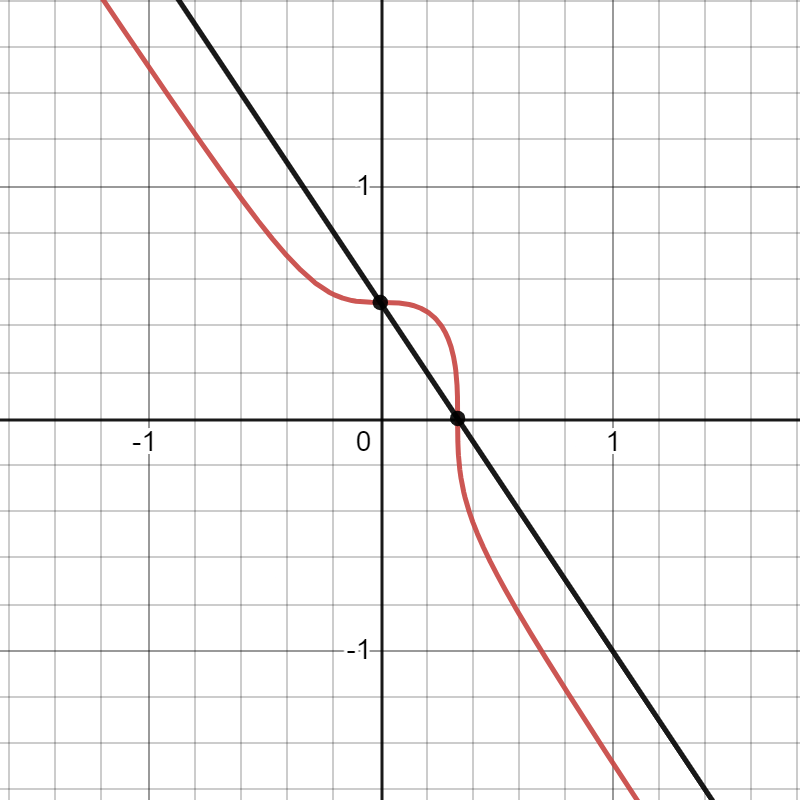
\includegraphics[width=0.5\textwidth]{desmos-graph (1).png}
\caption{\label{fig:asymptote} A line projected through points $(0, \frac{1}{2})$ and $(\frac{1}{3}, 0)$ with the curve $27x^{3}+8y^{3}-1 \ = \ 0$}
\end{figure}

Have two only points of intersection, $(0, \frac{1}{2})$ and $(\frac{1}{3}, 0)$ but get asymptotically gets closer and closer. \\

However, thinking using our new projective space, we can see that a projective cubic curve contains "points at infinity" that we lose when we project our curve onto $Q^2$, where $Z = 0$, and intuitively, we can see that if there is a point $[X : Y : 0] \in C(Q)$, then the $X$ to $Y$ ratio of this point will be the same as the $x$ to $y$ ratio of the asymptotes of the curve (as when $Z$ approaches $0$, $x = \frac{X}{Z}$ and $y = \frac{Y}{Z}$ will approach infinity). This can be seen by how the corresponding homogeneous equations to our example,

\[2Y + 3X - Z = 0 \quad \text{ and } \quad 27X^{3}+8Y^{3}-Z^3 \ = \ 0 \] 

Have three points of intersection, $[0 : 1 : 2]$, $[1 : 0 : 3]$ and $[2 : -3 : 0]$\\

Thus, our notion about there being \emph{exactly} three points of intersection can be made rigorous as a corollary of Bézout's theorem, which states:\\

If $f$ and $g$ are homogeneous polynomials of degree $d_1$ and $d_2$ respectively, then in the complex projective $P_C^2$ they meet in exactly $d_1 d_2$ points (counting multiplicity).\\

Without going into the details too much, in our case we have a line of degree $1$ and a cubic of degree $3$, so they meet in $3$ points in $P_C^2$ counting multiplicities. However, similar to how non-real solutions to real-coefficiented polynomials come in complex conjugate pairs, our non-real points of intersection also come in complex conjugate pairs. This means that if we know two of our points of intersection are in $P_R^2$ then the third point of intersection must also be in $P_R^2$. Hence, if two of the points of intersection are in $P_Q^2$, then there must be a third point in $P_Q^2$ as well as a rational line will only meet a rationally-coefficiented cubic at points in $P_Q^2$.\\

So we can see that our binary operation $*$ is well-defined. In fact, we can visually see a couple of properties of it. Namely, for all $P$, $Q$ in $P_Q^2$:

- $P * Q = Q * P$

- $(P * Q) * Q = P$

Now, as mathematicians we ask the question we've been trained to ask: $(C(Q), *)$ a group? Unfortunately not; it is not hard to mentally verify that a unique identity element doesn't exist and that associativity won't hold. However, by studying this operation further, we \emph{will} be able to use it to construct a group law.\\

First, for three points, $P$, $Q$ and $R$ on our curve $C$ Write $P - Q - R$ to mean these three points are colinear, this notation helps us clear up the fact that these six statements are equivalent:

\[ P * Q = R, \ P * R = Q, \ R * P = Q, \ R * Q = P, \ Q * R = P \ \text{ and } \ Q * P = R \]

Using this new notation, we can concisely write out a theorem which describes a subtle but important property of $*$:\\

If, for some $A, B, C, D, E, F, G, H \in C(Q)$: 

$A - B - C$ and $D - E - F$ and $A - D - G$ and $B - E - H$

then $C * F = G * H$\\

Or, even more suggestively:
\[
\text{if} \qquad
\begin{matrix}
A & - & B & - & C\\
| &   & | & \\
D & - & E & - & F\\
| &   & | &\\
G &   & H &\\
\end{matrix}
\qquad \text{then, for some} \ J \in C(Q) \qquad
\begin{matrix}
A & - & B & - & C\\
| &   & | &   & |\\
D & - & E & - & F\\
| &   & | &   & |\\
G & - & H & - & J\\
\end{matrix}
\]

Although the notation makes this look intuitive, it is not at all obvious. Why should the line defined by $C$ and $F$ and the line defined by $H$ and $J$ intersect with the cubic curve at the same point? The first observation that we can make is that if we take the homogeneous equations of three projective lines, say:

\begin{align*}
    L_{11} X + L_{12} Y + L_{13} Z &= 0 \\
    L_{21} X + L_{22} Y + L_{23} Z &= 0 \\
    L_{31} X + L_{32} Y + L_{33} Z &= 0 \\
\end{align*}

Then, multiplied together, we can get the homogeneous equation of a cubic curve, which is simply the union of our three lines:

\[(L_{11} X + L_{12} Y + L_{13} Z)(L_{21} X + L_{22} Y + L_{23})(L_{31} X + L_{32} Y + L_{33} Z) = 0\]

Hence, we can see that, treating the three vertical lines in our diagram as one cubic and the three horizontal lines as another cubic, our theorem is a special case of the Cayley–Bacharach theorem, which states:\\

Three cubic curves that meet at eight points $P_1 \dots P_8$ will also all meet at a ninth point $P_9$.\\

Proof: let $\vec{a}, \vec{b}$ and $\vec{c}$ be the vectors containing the coefficients for some homogeneous cubics $a(X, Y, Z)$, $b(X, Y, Z)$, and $c(X, Y, Z)$ and let $M$ be a matrix containing the evaluations of each of the terms in a cubic polynomial at the points $P_i = [X_i : Y_i : Z_i]$:\\

\[ \vec{a} = 
\begin{bmatrix}
A_0 \\
A_1 \\
\vdots\\
A_9\\
\end{bmatrix} 
\vec{b} =
\begin{bmatrix}
B_0 \\
B_1 \\
\vdots\\
B_9\\
\end{bmatrix} 
\vec{c} = 
\begin{bmatrix}
C_0 \\
C_1 \\
\vdots\\
C_9\\
\end{bmatrix} ,
M = 
\begin{bmatrix}
X_1^3  & Y_1^3  & \dots  & X_1 Y_1 Z_1 \\
X_2^3  & Y_2^3  & \dots  & X_2 Y_2 Z_2 \\
\vdots & \vdots & \ddots & \vdots\\
X_8^3  & Y_8^3  & \dots  & X_8 Y_8 Z_8 \\
\end{bmatrix} 
\]

As all our points are on the curve:

\[M\vec{a} = M\vec{b} = M\vec{c} = \vec{0} \ \text{ or equivalently, } \ \vec{a}, \vec{b} \text{ and } \vec{c} \text{ are in the kernel of }M,  ker(M) \]

Now, as a consequence of our points being distinct, all of $M$'s rows are linearly independent, so $M$ has a rank of $8$. By the rank-nullity theorem, this means that the dimension of the kernel of $M$ must be $2$, telling us that $\vec{a}$, $\vec{b}$ and $\vec{c}$ must be linearly dependent. As $\vec{a}$ and $\vec{b}$ are non-zero for them to actually describe cubic curves, this means that we should be able to find constants $\lambda_1$ and $\lambda_2$ such that:\\

\[\vec{c} = \lambda_1 \vec{a} + \lambda_2 \vec{b}\]

so, for all $[X : Y: Z] \in P_Q^2$:

\[c(X, Y, Z) = \lambda_1 a(X, Y, Z) + \lambda_2 b(X, Y, Z)\]

Hence, for any ninth point of intersection $P_9 = [X_9 : Y_9 : Z_9]$ of the curves defined by $a$ and $b$, $a(X_9, Y_9, Z_9) = 0$ and $b(X_9, Y_9, Z_9) = 0$ as $P_9$ is on both these curves, however this means that $c(X_9, Y_9, Z_9) = 0$ so $P_9$ is on the curve defined by $C$ too, completing our proof. \\

While this theorem is interesting, we still need to examine what it means for our binary operation $*$ to make any use of it. Note that the proposition of our theorem involves eight points, however only four of our points are "free". Hence, it makes sense to re-write our result that $G * H = C * F$ to say:

\[(A * D) * (B * E) = (A * B) * (D * E) \quad \text{for any} A, B, D, E \in C(Q)\]

This kind of hints that there may be some form of associative operation that we can wrangle out of our result. Namely, if we instead let $D$ be dependent on $A$ and $G$ and $B$ be dependent of $A$ and $C$, our theorem is:

\[G * ((A * C) * E) = C * ((A * G) * E) \quad \text{for any} A,  C, E, G \in C(Q)\]

We can now finally see that, if for any $P, Q \in P_Q^2$, if we write $P + Q = (P * Q) * E$ for a fixed $E$. Then:

\[G * (A + C) = C * (A + G)\]

So, taking $* E$ on both sides gives:

\[G + (A + C) = C + (A + G)\]

It is not too tricky to see that our new $+$ relation inherits commutativity from $*$; so this above statement can be converted into saying that $+$ is associative:

\[P + (Q + R) = (P + Q) + R \quad \text{ for any } P, Q, R \in C(Q)\]

In defining our operation $+$, we chose a fixed point $E$ on $C(Q)$. From now on, we will refer to this point as $\mathbf{0}$, as it satisfies the identity property:

\[P + \mathbf{0} = (P * \mathbf{0}) * \mathbf{0} = P \quad \text{ for any } P \in C(Q)\]

All we need to do now to show that $(C(Q), +)$ is a group is to is show that there are inverse elements. Let $P \in C(Q)$. Then we want $-P$ to have the property that:

\[ P + (-P) = (P * (-P)) * \mathbf{0} = \mathbf{0}\]

Hence, we can see that we want:

\[P * (-P) = \mathbf{0} * \mathbf{0} \]

So we can see that we can find $P$'s additive inverse with the formula: $-P = P * (\mathbf{0} * \mathbf{0})$ .\\

Working with $+$ will turn out to be much easier than working with $*$ when in comes to studying $C(Q)$, specifically because it is an abelian group. One thing that feels slightly unnatural about our construction of $+$ is that it requires us to pick a point $\mathbf{0}$ on our curve $C(Q)$, however it turns out that all choices of $\mathbf{0}$ will give groups which are isomorphic to each other (the proof is relatively straightforwards, and can be seen at the end of Silverman section 1.2). Hence, it makes sense to talk about \emph{the} group of rational points $C(Q)$.

\subsection{The Weierstrass normal form}

Now that we have developed a theory of projective transformations and a theory of cubic curves, the natural question to ask is:\\

What happens when we apply projective transformations to cubic curves? Can we use projective transformations to simplify their equations?\\

In fact, we will see that, working in $P_Q^2$, all cubic curves can be projectively transformed into a type of cubic curve called an \emph{elliptic curve}, that has an equation in the \emph{wierstrauss normal form}. It is much easier to give an example of doing this transformation if we start with a rational point of multiplicity three, however there is a more complex method one can use on cubic curves where one doesn't have a rational point of multiplicity three, which can be found in Silverman.\\

Let us start with the cubic curve defined in non-homogeneous coordinates by:

\[ x^{3} - 4 x^{2} y - 4 x^{2} - 2 x y^{2} - 2 x y - 3 y^{3} - 5 y^{2} - 2 y\ =\ 0 \]

We will show that this curve can be transformed, using only projective transformations, into the much simpler elliptic curve:

\[y^2 = x^3 - x + 1\]

The first key is to see that our cubic curve has a point of multiplicity $3$ at [0: -1: 1], whereas our elliptic curve has a point of multiplicity $3$ at [0: 1: 0]. Hence, it makes sense that we should find a transformation that maps the former point to the latter point. A straightforwards transformation we could pick is:

\[ T_1 = \begin{bmatrix}
    1 & 0 & 0\\
    0 & -1 & 0\\
    0 & 1 & 1
\end{bmatrix},
\quad
T_1: <X, Y, Z> \; \mapsto \; <X, -Y, Y + Z>
\]

Subbing this to our equation gives:

\[x^{3} - 4 x^{2} + 2 x y - y^{2} + 2 y = 0\]

Equivalently:

\[y^2 - 2 x y - 2y = x^3 + 4x^2\]

As we see, our curve has been significantly simplified, however it still has some pesky $xy$ and $y$ terms that means that it doesn't have the nice symmetry about the $y$ axis that our target curve has. To get it in the desired form, we complete the square of the right hand side to see how we should transform our y coordinate.

\[(y - (x + 1))^2 - (x + 1)^2 = x^3 + 4x^2\]

Hence, it makes sense to pick a transformation that maps $y - (x + 1) \mapsto y$. One good candidate is:

\[ T_1 = \begin{bmatrix}
    1  & 0 & 0\\
    -1 & 1 & -1\\
    0  & 0 & 1
\end{bmatrix},
\quad
T_2: <X, Y, Z> \; \mapsto \; <X, Y - X - Z, Z>
\]

After this transformation, our curve has equation:

\[y^{2} = x^{3} - 3 x^{2} + 2 x  + 1\]

This curve is already in the "Weierstrass normal form"; however we can simplify it even further. Namely, we know that the $x^2$ term ($-3$) is the sum of the roots of the cubic on the right, so if we apply a transformation that maps $T_3: x \mapsto x - 1$. This gives us the final equation of our curve:

\[y^{2} = x^{3} - x  + 1\]

\begin{figure}
\centering
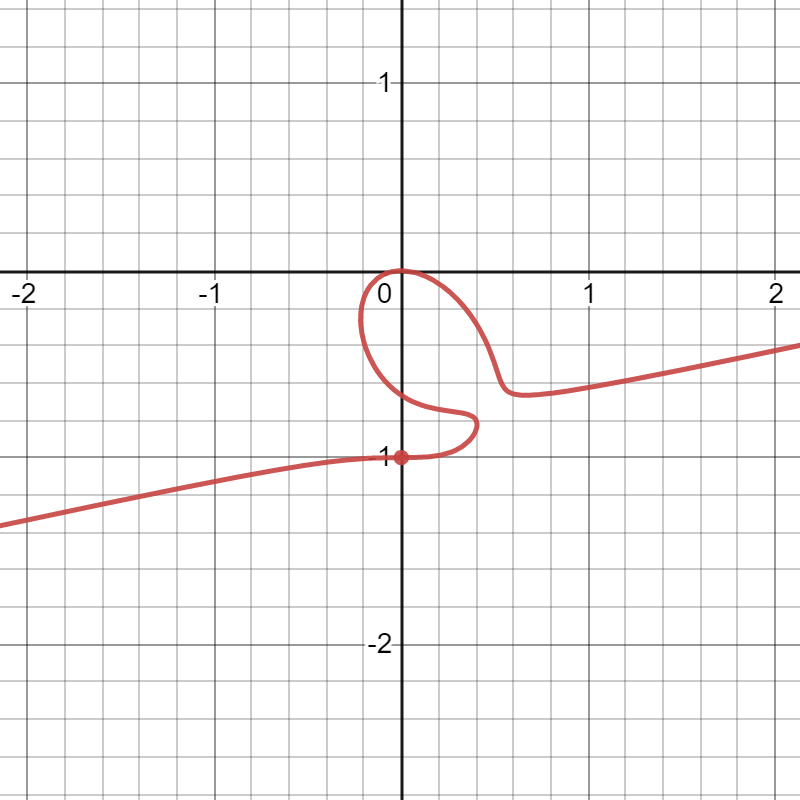
\includegraphics[width=0.3\textwidth]{desmos-graph (2-0).png}
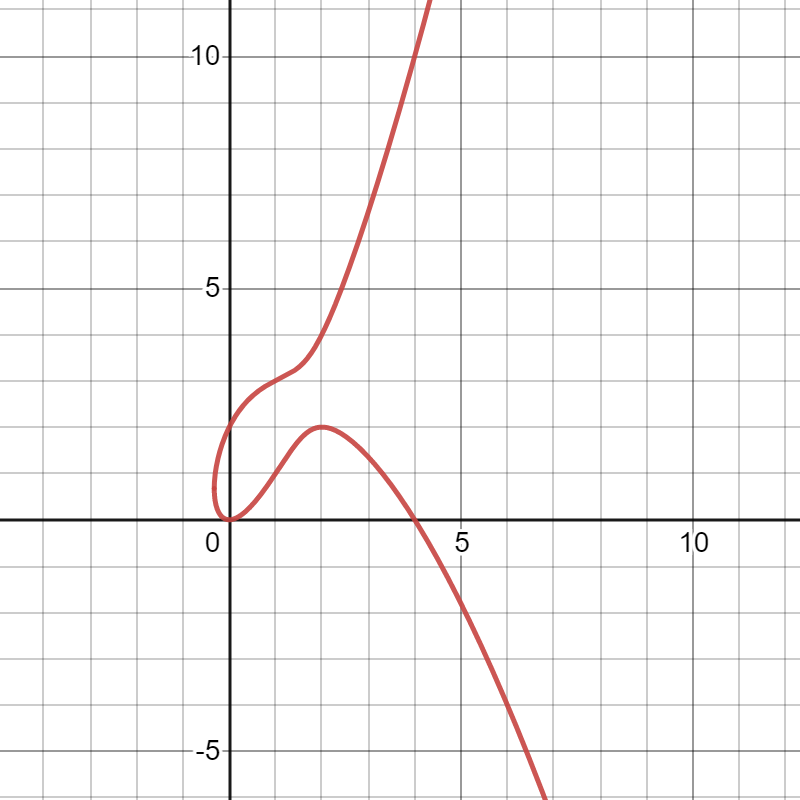
\includegraphics[width=0.3\textwidth]{desmos-graph (2-1).png}
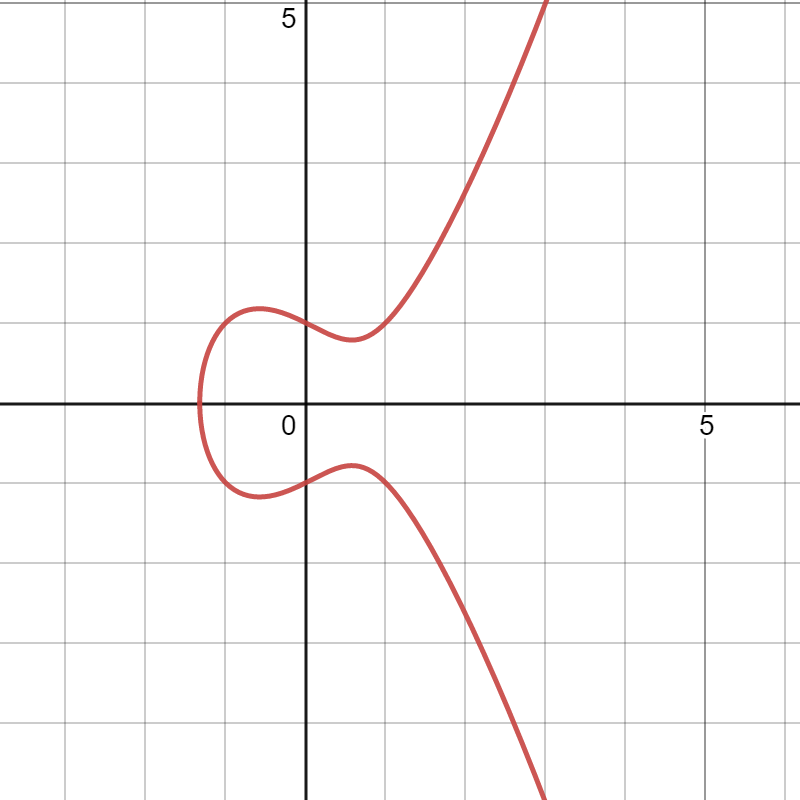
\includegraphics[width=0.3\textwidth]{desmos-graph (2-3).png}
\caption{\label{fig:into curve} Three steps of transforming our cubic curve into an elliptic curve.}
\end{figure}

This process can be replicated for \emph{any} cubic curve where we have a point of multiplicity three, which may be projectively transformed into an elliptic curve of the form:

\[y^2 = x^3 + bx + c\]

While this is interesting, it is not clear why it is important. The first thing to note is that we can combine our projective transformations into one  projective transformation $T = T_3 T_2 T_1$ which maps rational points on our original cubic curve $C(Q)$ to rational points on our elliptic curve $E(Q)$. As all projective transformations are invertible, this means that $T$ is in fact a bijection, so any rational point on $C(q)$ can be converted into a rational point on $E(Q)$ and vice versa. On top of this, we know that projective transformations map lines to lines, meaning that for any points $P$ and $Q$ on $T(P *_C Q) = T(P) *_E T(Q)$. Extending this a bit further, it is not tricky to see that it must be the case that:

\[T(P +_C Q) = T(P) +_E T(Q)\]

Hence, we can see that not only is T a bijection between the rational points of our curve, but it is in fact an \emph{isomorphism} between the groups of rational points. This means that anything we discover about the group of rational points of our simpler elliptic curve can be extended to all cubic curves, and we will see it will be easier to work with elliptic curves, mainly because it is much easier to add points on elliptic curves.

Specifically, if we pick $\mathbf{0}$ to be the point of multiplicity three $[0 : 1 :0]$ which is now the only "point at infinity" on our curve; then we can see that taking $P * \mathbf{0}$ just amounts to reflecting $P$ on the $x$-axis. Hence, for any points $P = (x_P, y_P)$ and $Q = (x_Q, y_Q)$ on an elliptic curve defined by the Weierstrass equation:

\[y^2 = f(x) = x^3 + ax^2 + bx + c\]

To calculate $P + Q$, we just need to find the $x$ and $y$ coordinates of $P * Q$ and then take the negative of the $y$ coordinate. It is thus not too hard to derive explicit formulae for adding points:

\[x_{P+Q} = x_{P*Q}, \quad y_{P+Q} = - y_{P*Q}\]

\[x_{P*Q} = \lambda^2 - a - x_P - x_Q \quad \text{ where } \quad \lambda = \begin{cases} 
          \frac{y_P - y_Q}{x_P - x_Q} & x_P \neq x_Q \\
          \frac{f'(x_P)}{2y_P} & x_P = x_Q \\
       \end{cases}\]
       
\[y_{P*Q} = \lambda x_{P*Q} + v \quad \text{ where } \quad v = y_P - \lambda x_P\]

Note that, as our $\mathbf{0}$ point has multiplicity two, $\mathbf{0} = \mathbf{0} * \mathbf{0}$, So to calculate the coordinates of $-P$, we just need to reflect about the $x$-axis too:

\[x_{-P} = x_P, \quad y_{-P} = -y_P\]

For example, suppose we have the points $P = (0, -1)$ and $Q = (1, 1)$ on the curve which we have computed:

\[y^{2} = x^{3} - x  + 1\]

To compute $P + Q$, we first find the equation line between our points:

\begin{figure}
\centering
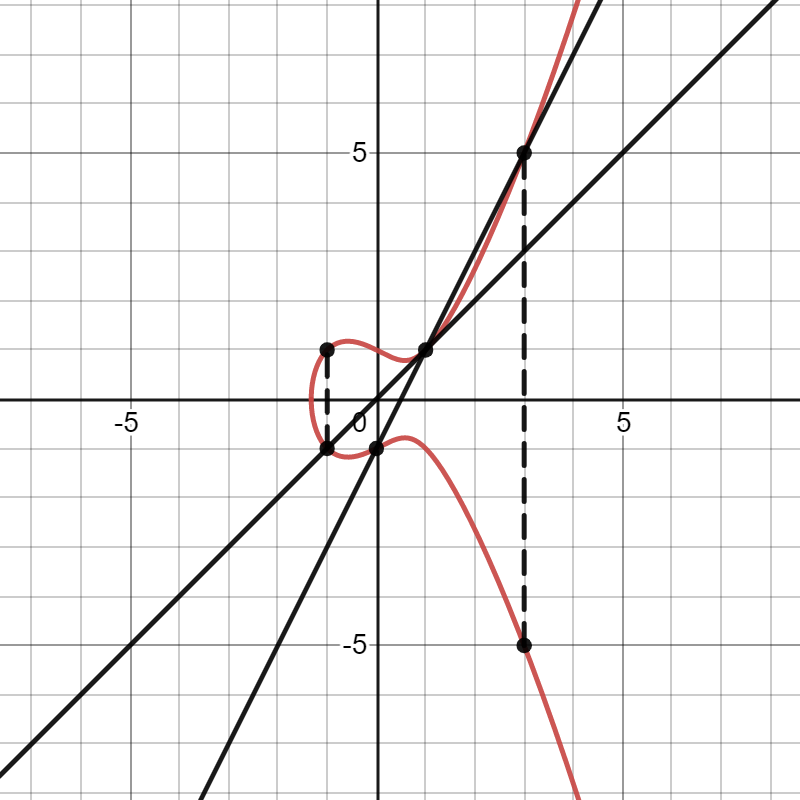
\includegraphics[width=0.5\textwidth]{desmos-graph (3).png}
\caption{\label{fig:into curve} $2Q$ and $P+Q$ calculated on the curve $y^{2} = x^{3} - x  + 1$}
\end{figure}


\[y = \lambda x + v \quad \text{ with } \quad \lambda = \frac{-1 - 1}{0 - 1} = 2, \quad v = 2\times 0 -1 = -1\]

Subbing this line equation for $y$ into our cubic will give us a cubic where, by examining the $x^2$ term, we can see the third root will be given by:

\[x_{P*Q} = \lambda^2 - 0 - 1 = 4 - 1 = 3\]

Subbing this into our line equation gives:

\[y_{P*Q} = 2 \times 3 - 1 = 5\]

Finally, reflecting about the $y$ axis gives $P + Q = (3, -5)$. To calculate $2Q$, we need to find the equation of the tangent at $Q$, namely:

\[y = \lambda x + v \quad \text{ with } \quad \lambda = \frac{f'(1)}{2 \times 1} = 1, \quad v = 1 \times 1 - 1 = 0\]

We can then repeat the same process as before to see: $2Q = (-1, -1)$

This whole process is much easier than trying to compute the sum $T^{-1}(P) \ + \ T^{-1}(Q)$ on our original cubic.

\newpage


\section{Mordell's theorem}

In this section we will go over a theorem originally proved by Louis Mordell in 1922, which states that the group of rational points over any elliptic curve $C(Q)$ is finitely generated; ie there exists some finite subset of $C(Q)$ such that every element of $C(Q)$ can be written as the sum of points in this subset. This tells us alot about the group's structure; namely using the fundamental theorem of finitely generated abelian groups it tells us that:

\[C(Q) \cong Z^n \times C(Q)_{tors}\]

Where $C(Q)_{tors}$ is the finite subgroup of \emph{torsion points} of $C(Q)$ (the points of finite order) and $n$ is called the \emph{rank} of our Elliptic curve. The question of what possible ranks elliptic curves can have is still an open question; with no clear conjecture as to what the answer should be. A similar proof was extended by Wiel to the Mordell-Wiel thoerem for his doctoral thesis; this theorem states that all abelian varieties (of which elliptic curves are a type) have finitely generated sets of rational points.\\

For brevity, I have emitted the proof for one of the key lemmas in the theorem (namely that there is a finite number of cosets of $2C(Q)$ in $C(Q)$) because fully proving it would require a significant detour into complex analysis. Other lemmas I have only partially proved; hoping to give an intuition as to why the fact is true rather than getting into the weeds of writing out a full proof - which would make this report much longer than I am targeting. Full proofs for all these lemmas can be found in Silverman.\\

One thing one will notice by playing around with the addition law is that, as we add points, the points seem to get progressively more "complex" (in the sense of how much information is needed to store the point's coordinates, \emph{not} in the sense of complex numbers). For instance: \\

Take $C(Q)$ to be the ellipic curve defined by:

\[ y^2 = x^3 + 3x^2 + x - 1 \quad \text{with} \quad P = (-2, 1)\]

Then, using python to compute $nP$ we see:

\begin{align*}
    1P &= \left(-2,1 \right) \\ 
    2P &= \left(\frac{5}{4},- \frac{21}{8} \right) \\ 
    3P &= \left(- \frac{170}{169},\frac{239}{2197} \right) \\ 
    4P &= \left(\frac{5713}{7056},\frac{900271}{592704} \right) \\ 
    5P &= \left(- \frac{4129274}{2325625},- \frac{3693595151}{3546578125} \right) \\
    6P &= \left(\frac{3224423333}{38613796},\frac{186368366079819}{239946128344} \right) \\ 
    & \ \ \vdots
\end{align*}



Hence, it makes sense that our generating set would be comprised of points of low complexity (and as the generating set is finite, at least \emph{bounded} complexity), to prove our theorem about $C(Q)$ being finitely generated; it makes sense to do two things;\\

1. prove that the number of points below a certain bound of complexity is finite \\

2. show that every point can be decomposed into a sum of lower-complexity points \\

To do this, we define the \emph{height} of a rational number $q = \frac{m}{n}$ as the maximum of it's numerator and denominator written in it's lowest terms:

\[ H(q) = H\left(\frac{m}{n}\right) = max(|m|, |n|) \text{where m and n are coprime.} \]

We will see that we can adapt this notion of height of rational numbers into a concrete measure of complexity for our points. But first, we need to examine height in more detail.

\subsection{The properties of height}

To get familiar with the height function, one can mentally verify that the height function sastisfies the following upper bounds:\\

- $ H(pq) \ \leq \ H(p)H(q) $\\

- $ H(p + q) \ \leq \ 2H(p)H(q) $\\

- $ H(p^n) \ = \ H(p)^n $ \\

As our formulae for adding points involves substituting their coordinates in for polynomials; it makes sense to examine how the height works with polynomials. Intuitively, it makes sense that the the size numerator or denominator of the result of a polynomial will grow roughly with the size of the numerator or denominator of the input raised to the degree of the polynomial; which we can express with the following lemma:\\

If $f$ is a polynomial of degree $n$, then there exist constants $K_l$ and $K_u$ only depending on $f$ such that, for all $x$:

\[ K_l (H(x))^n \leq H(f(x)) \leq K_u (H(x))^n \]

The proof of the upper bound is relatively straightforwards using our upper bound properties of height:

\begin{align*} 
H(f(x)) &= H(a_n x^n + a_{n-1}x^{n-1} + \dots + a_1 x + a_0)\\
&\leq 2H(a_n x^n + a_{n-1}x^{n-1} + \dots + a_1 x)H(a_0)\\
&\leq 2H(x(a_n x^{n-1} + a_{n-1}x^{n-2} + \dots + a_1))H(a_0)\\
&\leq 2H(x)H(a_n x^{n-1} + a_{n-1}x^{n-2} + \dots + a_1)H(a_0)\\
&\leq 4H(x)H(a_n x^{n-1} + a_{n-1}x^{n-2} + \dots)H(a_1)H(a_0)\\
&\dots\\
&\leq 2^n (H(x))^n H(a_n)H(a_{n-1})\dots H(a_1)H(a_0)
\end{align*} 

then, we can see that:

\[ H(f(x)) \leq K_u H(x)^n \quad \text{with} \quad K_u = 2^n H(a_n)H(a_{n-1})\dots H(a_1)H(a_0) \]

Proving the lower bound is trickier, mainly because for arbitrary $p$ and $q$ we cannot put lower bounds on $H(pq)$ or $H(p + q)$ based solely on $H(p)$ and $H(q)$. Instead, we have to write $x = \frac{\alpha}{\beta}$ as a fraction in it's lowest terms. Then, we can see that:

\begin{align*}
    H(f(x)) &= H(f(\frac{\alpha}{\beta}))\\
            &= H(\frac{1}{\beta^n}(a_n \alpha^n + \alpha_{n-1} \beta x^{n-1} + \dots + a_1 \alpha \beta^{n-1} + a_0 \beta^n))\\
            &= max(|\beta^n|, |\beta^n f(\frac{\alpha}{\beta})|)\
\end{align*}

On the last line, we used the fact that both $\beta^n f(\frac{\alpha}{\beta})$ and $\beta^n$ are integers, and that $\beta^n f(\frac{\alpha}{\beta}) - \alpha^n \equiv 0 \quad (\bmod{\beta})$ but $\alpha \not\equiv 0 \quad (\bmod{\beta})$, so $gcd(\beta^n f(\frac{\alpha}{\beta}), \beta) = 1$. Now, as the max of two numbers is always greater than the average, we can see that:

\begin{align*}
    H(f(x)) & \geq \frac{|\beta^n| + |\beta^n f(\frac{\alpha}{\beta})|}{2}\\
    &\text{so}\\
    \frac{H(f(x))}{H(x^n)} &\geq \frac{|\beta^n| + |\beta^n f(\frac{\alpha}{\beta})|}{2 max(|\alpha^n|,|\beta^n|)}\\
                        &= \frac{1 + |f(\frac{\alpha}{\beta}|)}{2 max(1, |\frac{\alpha^n}{\beta^n}|)}\\
                        &= \frac{1 + |f(x)|}{2 max(1, |x|^n)}
\end{align*}

Hence, all we need to do to prove our lemma is show that the function: $g(x) = \frac{1 + |f(x)|}{2 max(1, |x|^n)}$ has positive lower bound $g(x) \geq K_l > 0$. Note that this function is continuous, so it's image is a interval in $R$. Let $K_l = inf(im(g)$, it suffices to show that $K_l > 0$. Note that $g$ is positive, so $K_l \geq 0$ so the only case we have to deal with is when $K_l = 0$. in this case, $g$ gets arbitrarily close to $0$ so we must be able to find a convergent sequence $(x_n)$ such that $g(x_n) \rightarrow K_l = 0$. \\

- In the case where $(x_n)$ converges to some real number $r$ we can see that as $g$ is continuous, $g(r) = 0$, which we can see is a contradiction as $g$ is a strictly positive function.\\

-In the case where $(x_n)$ converges to $\infty$, we can see that $g(x) \rightarrow \frac{|a_n|}{2}$, which must be non-zero as $a_n$ is non-zero, so we also derive a contradiction.\\

Thus, conclude the proof of our lower bound:

\[ K_l H(x)^n \leq H(f(x)) \]

Notationally, it becomes easier to examine the log-height, denoted with a small $h$: $h(x) = ln(H(x))$. Then our lemma becomes:

\[ n h(x) + k_l \leq h(f(x)) \leq n h(x) + k_u \]

Applying this lemma to our curve, we can see there exists constants $k_1$ and $k_2$ such that if $(x, y)$ is a point the curve: $y^2 = f(x) = x^3 + ax^2 + bx + c$:

\[ \frac{3}{2} h(x) + k_1 \leq h(y) \leq \frac{3}{2} h(x) + k_2 \quad \text{as} \quad h(y) = \frac{1}{2}h(f(x)) \]

Hence, for a point $P = (x_P, y_P) \in C(Q)$ it makes sense to define the complexity of $P$ as the height of it's $x$ coordinate, as the height of it's $y$ coordinate is linked to the height of it's $x$ coordinate and it is easier to compute the $x$ coordinates of $2P$ and $P + Q$. From now on, we will denote $h(P) = h(x_P)$ to be the height of the \emph{point} $P$. By convention, we also set $h(0) = 0$.\\

Before doing this, we will prove a lemma that will be key to our theorem:\\

For any given curve $C(Q)$ and upper bound $B$, there are only finitely many points $P \in C(Q)$ such that $h(P) < B$.\\

The proof is very simple; the trick is to think of the rational numbers as a plane where the denominator is plotted on the x axis and the numerator is plotted on the y axis. Consider the function $g: Z \times N \rightarrow Q$ where $g: (m, n) \mapsto \frac{m}{n}$. We can see that $g$ is surjective the set of inputs to $g$ which give an output with height less than $B$ is a rectangle, with one side length $2B + 1$ (as there are $2B + 1$ choices for the numerator) and the other side length $B$ (as there are $B$ choices for the denominator). Hence, there are at most $B(2B + 1)$ distinct rational numbers with height less than $B$. However, for a given curve $C(Q)$, there are at most two points with a given rational $x$ coordinate, hence there are at most $2B(2B + 1)$ points of height less than $B$\\


To bring this back to what we said in our introduction, this means all we need to do to prove $C(Q)$ is finitely generated is to show that there is a set of points that generates $C(Q)$ and has bounded height; as then this set must be finite. Before we do this however, we need to examine how height interacts with the group law; as we need to introduce the notions of adding points with our height function for any hope of such a proof working.\\

\subsection{Examining how height interacts with the group law}

Let $P = (x_P, y_P)$ be any point on an Elliptic Curve $C(Q)$. We will first examine how $h(2P)$ and $h(P)$ relate.\\

Recall we can re-write our formula for $x_{2P}$ such that it is only in terms of $x_P$:

\[x_{2P} = \frac{f'(x_P)^2}{4 f(x_P)} - a - 2x_P = \frac{x_P^4 - 2bx_P^2 - 8cx_P + b^2 - 4ac}{4(x_P^3 +x_P^2 + bx_P + c)}\]

In the first section, we derived a result about the height of polynomials in terms of the height of the input variable; we will see that we can derive a similar result for the \emph{quotients} of polynomials as well. Namely, if $p(x)$ is a polynomial of degree $n$ and $q(x)$ is a polynomial of degree less than $n$ without common roots to $p$ (to prevent cancellation), then the height of $\frac{p(x)}{q(x)}$ grows roughly with the height of $x^n$. In precise terms there exist $k_l$ and $k_u$ dependent only on $p$ and $q$ such that for all $x$;

\[n h(x) + k_l \leq h \left( \frac{p(x)}{q(x)} \right) \leq n h(x) + k_u \]

The proof is similar to the proof for just one polynomial; however it is much longer so I have not included it (One can see Section 3.3 of Silverman for the full proof). Applying this to our duplication formula gives:

\[4h(P) + k_l \leq h(2P) \leq 4 h(P) + k_u\]

This is our first result about the height of points under the group law. Now, we will let $Q = (x_Q, y_Q)$ be a point on $C(Q)$ and see how $h(P + Q)$ relates to $h(P)$.

\begin{align*}
    x_{P + Q} &= \lambda^2 - a - x_P - x_Q\\
              &= \frac{(y_P - y_Q)^2 - (x_P - x_Q)^2(a + x_P + x_Q)}{(x_P - x_Q)^2}
\end{align*}

Note that if we replace $y_P^2$ with $x_P^3 + a x_P ^2 + b x_P + c$ and eliminate then our numerator can be reduced to:

\[x_{P + Q} = \frac{A y_P - (B x_P^2 + C x_P + D)}{(x_P - x_Q)^2}\]

Where $A$, $B$, $C$ and $D$ can be written in terms of $a$, $b$, $c$, $x_Q$ and $y_Q$. As we know $y_P \approx x_P^{\frac{3}{2}}$, it makes sense to say that the numerator is roughly quadratic in $x_P$. Although we will not fully prove this, using the fact about the height of quotients of polynomials above we are lead to think that $H(x_{P+Q}) \approx K_Q H(x_P)^2$ where $K_Q$ depends on $Q$ as well as the coefficients of our curve. This turns out to be correct, with the final result being that there is a $k_Q$ dependent on $Q$ such that for all $P \in C(Q)$:

\[h(P + Q) \leq 2h(P) + k_Q\]

Again fully proving this - while not requiring particularly advanced mathematics - would take a couple pages of working; and this can be seen in Section 3.4 of Silverman if one wishes.

\subsection{Proving the descent theorem}

Thus far, we have three results that we will use in our proof:\\

- For any elliptic curve $C(Q)$ and  real number $B$, the number of points $P \in C(Q)$ such that $h(P) \leq B$ is finite.\\

- We have a lower bound $h(2P)$, namely that there is a $k$ only dependent on $C(Q)$ such that for any point $P \in C(Q)$ :

\[ 4h(P) - k \ \leq \ h(2P) \]

- We have an upper bound on $h(P + Q)$, namely that for all $Q \in C(Q)$ there is a $k_Q$ independent of $P$ such that:

\[ h(P + Q) \ \leq 2h(P) \ + k_Q \]

- As mentioned in the introduction to this section, there is one final lemma needed to prove Mordell's theorem; namely that there is a finite set $A = {A_1, A_2 ... A_N}$ such that every $P \in C(Q)$ can be written as :

\[ P = 2Q + A_i \quad \text{for some} \ i \]

This is equivalent to the statement that the image of the mapping $P \mapsto 2P$ (which turns out to be a subgroup of $C(Q)$) has a finite number of cosets in $C(Q)$. As already mentioned, Mordell proved this using some interesting properties of the curve $C(C)$, and unfortunately I cannot go over the proof here as it it too long.\\

These four lemmas can be brought together to prove there is a bound $B \in R$ such that every $P \in C(Q)$ with $h(P) < B$ can be written as a sum of points $P = P_1 + P_2 + P_3 + \dots P_N$ such that $h(P_i) < h(P) - 1$. Recursively applying this to our points $P_i$, we see that we can eventually write $P$ as a sum of points in the finite set.\\

For a given $B$, let:

\[ C(Q)_B = \{P \in C(Q) | h(P) \leq B\} \]

We will prove this now. Let $P_0 \in C(Q)$. We know we can find an $A_i \in A$ and $Q$ in $C(Q)$ such that:

\[P_0 = A_i + 2P_1 \]

equivalently:

\[ 2P_1 = P_0 - A_i \]

Applying our lower and upper bounds we see that:

\[ 4h(P_1) - k \quad \leq \quad  h(2P_1) =  h(P_0 - A_i)  \quad  \leq  \quad  2h(P_0) + k_{-A_i} \]

Hence:

\[ h(P_1) \ \leq \ \frac{1}{2}h(P_0) + \frac{1}{4} (k + k_{-A_i}) \]

Hence, if we let $k_A = \max_{A_i \in A}(k_{-A_i})$, which we know exists as $A$ is finite, we can see that if $\frac{1}{4}(k + k_A) \leq \frac{1}{2}h(P_0) - 1$ then:

\[ h(P_1) \leq \frac{1}{2}h(P_0) + \frac{1}{4} (k + k_{-A_i}) \leq \frac{1}{2}h(P_0) + \frac{1}{2}h(P_0) - 1 \leq h(P_0) - 1 \]

We can also see that the restriction $\frac{1}{4}(k + k_A) \leq \frac{1}{2}h(P_0) - 1$ can be turned into $h(P_0) \geq B$ where $B = \frac{1}{2}(k + k_A) + 2$. we have hence proven that: if $P_j \in C(Q)$ then either: $h(P_j) \leq B$ or we can find a $P_{j + 1}$ such that $h(P_{j + 1}) \leq h(P_j) - 1$ and $P_j = 2P_{j+1} + A_i$ for some $A_i \in A$.\\

We can apply this reasoning inductively to show that, for any given $P_0 \in C(Q)$, we can eventually find a $P_N \in C(Q)$ and $A_{i_1}, A_{i_2} \dots A_{i_N} \in A$ such that:

\[ P_0 = 2^N P_N + A_{i_1} + 2 A_{i_2} + \dots + 2^{N-1}A_{i_N} \]

\[ \text{and} \ h(P_N) \ \leq B. \ (\text{equivalently}, \ P_N \in C(Q)_B) \]

Hence, we can see that our two sets $C(Q)_B$ and $A$ can generate $C(Q)$; however, as $C(Q)_B$ and $A$ are finite, their union is finite, so $C(Q)$ is finitely generated.


\newpage

\section{The Nagell-Lutz theorem}

\subsection{General idea and motivation}

For this section, knowledge and familiarity with the concepts of rings and ideals asssumed\\

The Mordell-Wiel theorem gave us information about the structure of the group of rational points; however the problem of finding the rank or the generating set for some curve $C$ is still not fully solved. Thankfully, the other component of our group, the torsion subgroup, is much better understood, and in the following chapter we will go through a theorem that fully describes how to find all of it's points for any given curve C: the Nagell-Lutz theorem.\\

In general, points seem to increase their "complexity" when we add them. For instance, in our proof of the Mordell-Wiel theorem, we showed that the amount of points under some bound of the complexity measure of height was finite, and we could find a bound that contains all of the generating elements. This means that, if P is some generating element then the height of P must increase without bound, ie the sequence $h(nP)$ for natural $n$ is unbounded. This is in contrast to our points in the torsion group, where $h(nP)$ is periodic and therefore must be bounded. Hence, it seems like a good method to find the torsion points of our curve would be to look for points for which $h(nP)$ is bounded.\\

In fact, the description which the Nagell-Lutz theorem gives tells us that, if our curve has integer coefficients, then all of it's rational torsion points must have integer coefficients; ie if $T$ is the torsion subgroup then $T \subseteq C(Z)$. This is a strange and surprising result, and until we go through some of the basic lemmas of the proof, it is hard to intuitively explain why we would expect this to be the case. One thing we can see is that the complexity measure of height won't work for our proof: it is impossible to take $h(r)$ for some rational number $r \in Q$ and determine whether or not $r$ is an integer. At first, this may not seem like a big deal, however we will see later that it is not tricky to protectively transform \emph{any} elliptic curve into an elliptic curve with integer coordinates, and therefore by extension, \emph{any} cubic curve into an elliptic curve with integer coordinates.\\

The for some rational $r \in Q$ p-adic order of $r$, $ord_p(r)$ is defined as the value of the power of the prime $p$ when $p$ is completely "factored out" of $r$; ie, we can uniquely write:\\

$r = \frac{m}{n}p^v$ such that $p$, $m$ and $n$ are all coprime integers, then $ord_p(r) = v$\\

by convention, we define $ord_p(0) = \infty$ as in a sense $p$ divides $0$ infinitely\\

Knowledge of p-adic numbers is not necessary to understand the proof, however it does add to the intuitions one may have. This complexity measure has the nice property that $r$ is an integer if and only if $ord_p(r) \geq 0$ for all primes $p$, making it more suitable for the theorem that we are going to prove. \\

There are some other nice facts about p-adic order that one can mentally verify:\\

for all $q, r \in Q$:\\

- $ord_p(qr) = ord_p(q) + ord_p(r)$\\

- if $ord_p(q) = ord_p(r)$ then $ord_p(q + r)  \geq ord_p(q)$ or $ord_p(r)$\\

- if $ord_p(q) > ord_p(r)$ then $ord_p(q + r) = ord_p(r)$\\

- in general, $ord_p(q + r) \geq min(ord_p(q)$, $ord_p(r))$\\

We still don't have a measure that we can apply to points on $C(Q)$ just yet, but we can use these facts to prove a theorem about integer-coefficiented polynomials:\\

if $f(x) = x^n + c_{n-1}x^{n-1} + c_{n-2}x^{n-2} + \dots c_1 x + c_0$ is an integer coefficiented-polynomial, then for all $x \in Q$ with $ord_p(x) < 0$: $ord_p(f(x)) = n \ ord_p(x)$\\

The proof is relatively simple:

first, note that $ord_p(c_k x^k) = ord_p(c_k) + k \ ord_p(x)$ and that, as $f$ has integer coefficients, $ord_p(c_k) \geq 0$ hence $ord_p(c_k x^k) \geq k \ ord_p(x)$. However, as $ord_p(x) < 0$, $k \ ord_p(x) > n \ ord_p(x)$ for $k > n$. Hence we can see that $ord_p(c_k x^k) > ord_p(x^n)$ so our $x^n$ term will "eat" all the terms to the right of it:

\[ ord_p(x^n) = ord_p(x^n + c_{n-1}x^{n-1}) = ord_p(x^n + c_{n-1}x^{n-1} + c_{n-2}x^{n-2}) = \dots = ord_p(f(x)) \]


Thinking about this with respect to elliptic curves naturally leads us to the following corollary:\\

Let $C$ be an elliptic curve defined by $y^2 = f(x)$ for some integer coefficiented cubic $f$; Then, for all points $P = (x_P, y_P) \in C(Q)$ and all primes p; either:\\

\[ ord_p(x_P) \geq 0 \quad \text{and} \quad  ord_p(y_P) \geq 0 \]

\[ \text{or} \quad  2 \ ord_p(y_P) = 3 \ ord_p(x_P) \]

This is not too tricky to see:\\

if \quad $ord_p(y_P) < 0$ \quad then \quad $ord_p(f(x_P)) < 0$ \quad so \quad $ord_p(x_P) < 0$

and if \quad $ord_p(x_P) < 0$ \quad then \quad $3 \ ord_p(x_P) = ord_p(f(x_P)) = ord_p(y_P^2) = 2 \ ord_p(y_P)$\\

Hence, if $ord_p(x_P) < 0$ or $ord_p(y_P) < 0$ we should be able to find an integer $v > 0$ such that: $ord_p(x_P) = -2v$ and $ord_p(y_P) = -3v$\\

Applying this with all primes p tells us that $x_P$ and $y_P$ are of the form:\\

$x_P = \frac{m}{e^2}$ \quad and \quad $y_P = \frac{n}{e^3}$ for some integers $m$, $n$ and $e$\\

One way of defining a complexity measure for our points in $C(Q)$ for a given prime $p$ could be to say that $Complexity_p(P) = v$ where $v$ is the integer such that:  $ord_p(x_P) = -2v$ and $ord_p(y_P) = -3v$. We also need to extend this to points with that $ord_p(x_P) \geq 0$ and $ord_p(y_P) \geq 0$. To do this, we define $t(P) = \frac{x_P}{y_P}$ then we see that, using the definition of $v$ above, $ord_p(t(P)) = ord_p(x_p) - ord_p(y_P) = v$. \\ 

Unfortunately, we will see later that just by examining $t(P)$ it is impossible to tell if a point $P$ has integer coordinates. In order to have some way to keep track of this, we define subsets of points than have more than $2v$ or $3v$ factors of $p$ in their $x$ and $y$ coordinate's denominators:

\[ C(p^v) = \{(x, y) \in C(Q) \ | \ ord_p(x) \ \leq \ -2v \ \text{and} \ ord_p(y) \ \leq \ -3v\} \]

Then, to prove that a given point $P$ has integer coordinates, we just need to prove $P \notin C(p)$ for all primes $p$.\\

Note that $P \in C(p^v)$ implies $ord_p(t(P)) \geq v$ but not the other way round; take for instance this case where $p = 2$:\\

$P = (2, 3)$ is on the curve $y^2 = x^3 - x + 3$ and we can see $ord_2(t(P)) = ord_2(\frac{2}{3}) = 1$ but $P \notin C(2^1)$ \\

Now, given that both our $t$ function and our addition formula are defined completely algebraically over our sets of points, it makes sense that we may get some useful results from studying how they interact.

\subsection{Investigating the p-adic order of P + Q}

For this section, we will fix a certain prime $p$.

Let R be the ring of rational numbers with p-adic order greater than or equal to 0 (ie, the rationals which have powers of p only in their numerator if at all):

\[ R = \{r \in Q \; | \; ord_p(r) \geq 0\} \]

We can see that the units (elements in R with multiplicative inverses in R) are precisely the rationals with p-adic order 0. We can also see that the ideals of $R$ generated by $p^v$ for some $v$ are precisely the sets of rational numbers with p-adic order greater than than or equal to $v$:

\[ p^vR = \{r \in Q \; | \; ord_p(r) \geq v\} \]

Let $P$ and $Q$ both be in $C(p^v)$ for some $v$. We wish to study the p-adic order of the coordinates of $P + Q$ to see if we get anything interesting. As we saw in section 4.2, it is fruitful to define $t(P) = \frac{x_P}{y_P}$. We can see that we can actually make this value into a coordinate of P after applying a projective transformation $(x, y) \mapsto (t, s)$ given by:

\[ t = \frac{x}{y} \ \text{and} \ s = \frac{1}{y} 
\quad \text{described by matrix:} \quad \begin{bmatrix}
    1 & 0 & 0\\
    0 & 0 & 1\\
    0 & 1 & 0
\end{bmatrix}
\]

The important thing to note here is that $P \in C(p^v)$ iff $t_P \in p^v R$ and $s_P \in p^{3v} R$; so this transformation doesn't loose any information about whether or not $P$ is in $C(p^v)$\\

This transformation is it's own inverse, so $x$ and $y$ are given by:

\[ x = \frac{t}{s}, y = \frac{1}{s} \]

Plugging these into our curve's equation gives:

\[ \frac{1}{s^2} = \frac{t^3}{s^3} + a \frac{t^2}{s^2} + b \frac{t}{s} + c \]

hence:

\[ s = t^3 + a t^2 s + b t s^2 + c s^3 \]

\begin{figure}
\centering
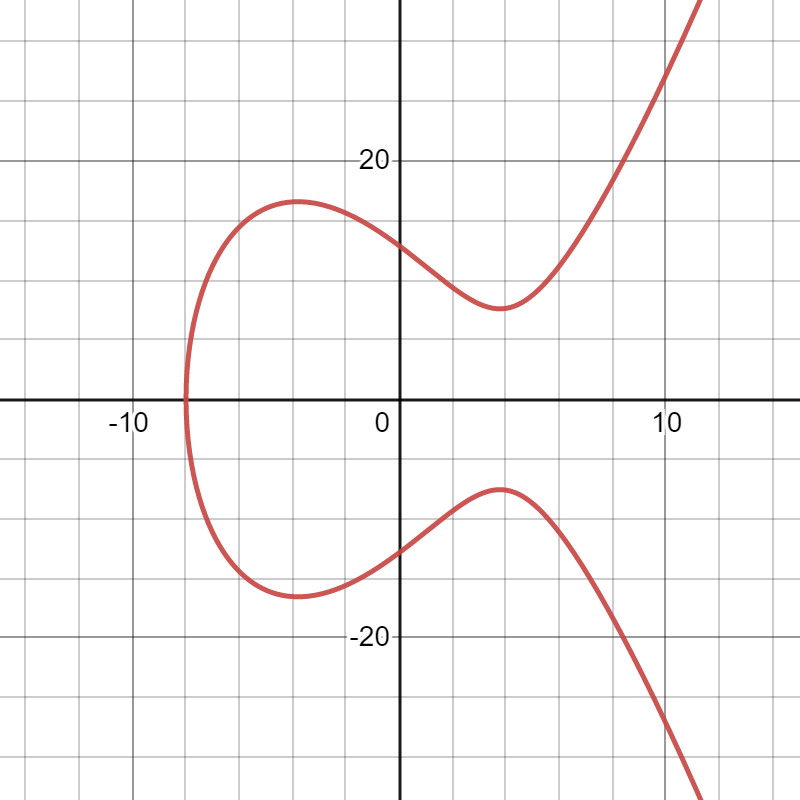
\includegraphics[width=0.3\textwidth]{desmos-graph (4).png}
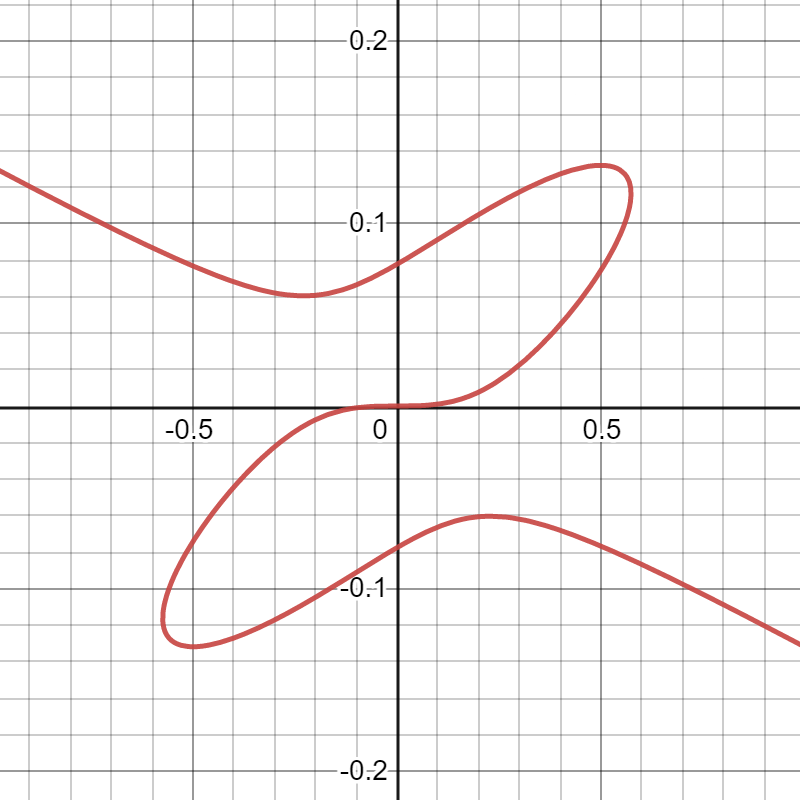
\includegraphics[width=0.3\textwidth]{desmos-graph (4-1).png}
\caption{\label{fig:into curve} The curve $y^2  = x^3 - 43 x + 166$ before and after being transformed into $s, t$ coordinates}
\end{figure}


Now, to add $(t_P, s_P)$ and $(t_Q, s_Q)$ on our curve we simply follow the procedure for a standard cubic curve.\\

First, we find the line going through $t_P$ and $t_Q$:

\[ s = \alpha t + \beta \quad \text{with} \quad \alpha = \frac{s_P - s_Q}{t_P - t_Q} \text{and} \beta = s_P - \alpha t_P \]

Then, we simultaneously solve the line equation and the curve equation to find the third intersection point:

\[ \alpha t + \beta = t^3 + a t^2 (\alpha t + \beta) + b t (\alpha t + \beta)^2 + c (\alpha t + \beta)^3 \]

Collecting terms gives:

\[ 0 = k_3 t^3 + k_2 t^2 + k_1 t + k_0 \]

where $k_3 = 1 + a \alpha + b \alpha^2 + c \alpha^3$ and $k_2 = a \beta + + 2 b \alpha \beta + 3c \alpha^2 \beta$\\

hence: 

\[ t_P + t_Q + t_{P*Q} = -\frac{k_2}{k_3} \]

Note that in our projective transformation the zero point was mapped to the origin and our curve is symmetric about the line $t + s = 0$ as if $(t, s)$ is on our curve then $(-t, -s)$ will also be on our curve. Combining these pieces of information, it is not too tricky to see that $(t_{P + Q}, s_{P + Q}) = (-t_{P * Q}, -s_{P * Q})$, hence we have that:

\[ t_P + t_Q - t_{P+Q} = -\frac{k_2}{k_3} \]

After this rather laborious bit of algebra, we can see a few things pop out at us: namely, if we can prove that $-\frac{k_2}{k_3} \in p^v R$ then we can prove that $t_{P+Q} \in p^v R$, strongly suggesting that $C(p^v)$ is a subgroup. Unfortunately, to get more information about $-\frac{k_2}{k_3}$ we must first go back and examine $\alpha$ and $\beta$. \\

As $s_P$ and $s_Q$ are in $p^{3v}R$ and $t_P$ and $t_Q$ are only in $p^v R$ it seems intuitive that $\alpha \in p^{2v}R$, however the preceding information alone doesn't give us enough information to \emph{prove} this. We need to also use the information that links $s_P$ with $t_P$ and $s_Q$ with $t_Q$; namely that they satisfy the cubic equation for our curve. Examining the top part of our fraction for $\alpha$, $s_P - s_Q$, gives:

\begin{align*} 
s_P - s_Q &= t_P^3 - t_Q^3 + a \; t_P^2 s_P - a \; t_P^2 s_P + b \; t_P s_P^2 - b \; t_Q s_Q^2 + c \; s_p^3 - c \; s_Q^3 \\
&= t_P^3 - t_Q^3 \\
& \quad + a(t_P^2 s_P - t_P^2 s_Q + t_P^2 s_Q - t_Q^2 s_Q) \\
& \quad + b(t_P s_P^2 - t_Q s_P^2 + t_Q s_P^2 - t_Q s_Q^2) \\
& \quad + c(s_P^3 - s_Q^3) \\
&= (t_P - t_Q)(t_P^2 + t_P t_Q + t_Q^2) \\
& \quad + a(s_P - s_Q)t_P^2 + a(t_P - t_Q)(t_P + t_Q)s_Q \\
& \quad + b(t_P - t_Q)s_P^2 + b(s_P - s_Q)(s_P + s_Q)t_Q \\
& \quad + c(s_P - s_Q)(s_P^2 + s_P s_Q + s_Q ^2)
\end{align*} 


Factoring out $s_P - s_Q$ and $t_P - t_Q$ gives:

\[(1 - A)(s_P - s_Q) = B(t_P - t_Q)\]
where 
\[A = a t_P^2 + b(s_P + s_Q)t_Q + c(s_P ^2 s_p s_Q + s_Q^2) 
\quad \text{and} \quad
B = (t_P^2 + t_P t_Q + t_Q^2) + a (t_P + t_Q)s_Q + b s_p^2\]

Hence: 

\[ \alpha = \frac{s_P - s_Q}{t_P - t_Q} = \frac{B}{1 - A} \]

Now, we can see that $B \in p^{2v}R$ and $A \in p^{2v} R$ from the fact that they are the sums of terms in these ideals. Hence, $ord_p(A) \geq 2v \geq 0 = ord_p(1)$ so $ord_p(1 - A) = 0$. Hence $1 - A$ is a unit in $R$ so $\frac{1}{1 - A} \in R$, meaning that we can conclude $\alpha = \frac{B}{1 - A} \in p^{2v}R$ \\

Now, going back to our formulas for $k_3$ and $k_2$ we see that and applying similar reasoning, $k_2 \in p^{3v}R$ and $\frac{1}{k_3} \in R$ so $\frac{k_2}{k_3} \in p^{3v}R$. This finally allows us to see that:

\[ t_P + t_Q - t_{P+Q} \in p^{3v}R \]

Written in modular arithmetic notation, this becomes even more suggestive that this is something that will be useful in our proof: 

\[ t_P + t_Q  \equiv t_{P+Q} \quad (\bmod{p^{3v}R}) \]

This shows that $t_{P+Q} \in p^{v}R$ but doesn't on it's own doesn't show that $P + Q \in C(p^v)$, we also have to show that $s_{P + Q} \in p^{3v}R$. This isn't too tricky; as $P*Q$ is on the same line as $P$ and $Q$:\\

\[s_{P*Q} = \alpha t_{P*Q} + \beta \in p^{3v}R \quad \ \text{ as } \ t_{P+Q}, \ \alpha \ \text{ and } \ \beta \ \text{ are in } \ p^v R, \ p^{2v} R \ \text{ and } \ p^{3v} R  \text{ respectively} \]

Hence, we also have that $s_{P+Q} = -s_{P*Q} \in p^v R$, so our set of points $C(p^v)$ is closed under addition of points. In fact, as $P*Q = - (P+Q)$ and we have also in the process shown $P*Q \in C(p^v)$, $C(p^v)$ is a subgroup of $C(Q)$. \\

To summarise the two main findings of our investigation:\\

- We have a series of of subgroups of rational points given by: $C(Q) \supseteq C(p) \supseteq C(p^2) \supseteq C(p^3) \dots$\\

- if $t_P$ and $t_Q$ are in $p^v R$ for some $v$, then: $t_P + t_Q  \equiv t_{P+Q} \quad (\bmod{p^{3v}R})$

\subsection{Finishing off the Nagell-Lutz proof}

Let $p$ be any prime number\\

Let $P \in C(Q)$ be a point of order $m$ with $m \neq 1$. We will show $P \notin C(p)$ \\

First, we need to factor most (or all) of the powers of $p$ in $m$ so that they don't interfere with our proof (We will see later why this is necessary).\\

It is not hard to see that for any $m \neq 1$ we can find a $\bar{m} \neq 1$ that divides $m$ and has at most one factor of $p$. For instance, if $m$ has no factors of $p$ we can pick $\bar{m} = m$ and otherwise we can pick $\bar{m} = \frac{m}{p^k}$

Now, let $P' = \frac{m}{\bar{m}} P$. We can see it suffices to prove $P' \notin C(p)$ as $C(p)$ is a subgroup\\

Let $v$ be the unique natural number such that: $P' \in C(p^v)$ but $P' \notin C(p^{v+1})$ \\

if $v = 0$, we are done as $P' \notin C(p)$. Hence we are restricted to examining the case where $v > 0$, and in this case we can deduce that $ord_p(t(P')) = v$ Now, we can examine $P'$ using the congruence relation:

\begin{align*}
    \text{first, note; } \quad & t(\bar{m}P') = t(mP) = t(0) = 0 \\
    \text{Hence, } \quad & \bar{m}t(P') \equiv t(\bar{m}P') \equiv 0 \quad (\bmod{p^{3v}R}) \\
    \text{Hence } \quad & \bar{m}t(P') \in p^{3v}R \\
\end{align*}

Now we see why we chose to examine $P'$ rather than $P$: if we got to this stage with $P$, we would not be able to say much in general as the number in front of $t(P)$ could be arbitrarily divisible by $p$, However, as $\bar{m}$ has at most one factor of p, we can say:

\begin{align*}
    & t(P') \in p^{3v-1}R\\
    \text{hence :} \quad & ord_p(t(P)) \geq 3v - 1 \\
    \text{however, we know :} \quad & ord_p(t(P)) = v\\
    \text{hence: } \quad & v \geq 3v - 1
\end{align*}

So we are forced to conclude $v = 0$, which is a contradiction as we were restricted to the case $v > 0$.

Hence, for all points of finite order $P$ with $mP = 0$; either:

- $m = 1$ in which case $P = 0$

- $m \neq 1$ in which case $P \notin C(p)$ for all primes $p$, so $P$ must have integer coordinates

\subsection{Further constricting the set of torsion candidates}

Let $P \neq 0$ be a point of finite order. We have proved that if $(x, y) = P$ then $x$ and $y$ must be integers; however this unfortunately still gives us an infinite search space of possible candidates of points that could be torsion points on the curve. Thankfully, it is not too tricky to restrict this set to a finite set.\\

First, we know that as $P$ is on the curve with integer coordinates, 

\[ y^2 = f(x) = x^3 + a x^2 + b x + c \]

equivalently,

\[ y^2 - c = x(x^2 + a x + b) \]

Hence, we can see that for any candidate $y$, $x$ must divide $y^2 - c$ to give an integer point on the curve. So all we need to find is a finite set of candidate $y$ values; which is described by the following lemma:\\

If $P = (x, y)$ is a point of finite order then $y$ divides the discriminant of $f$ or $y = 0$\\

There may be other restrictions that we can place on $y$, but this one turns out to be the easiest. First, note that if $P$ is of order one then $P = 0$ and if $P$ is of order two, then $P = -P$ which can only be the case if $y = 0$. Hence, we can restrict our search to the points where $P$ and $2P$ are both non-zero points of finite order (and hence both have integer coordinates).

\begin{align*}
    \text{Let } \quad & 2P = (x_2, y_2)\\
    \text{then, we have: } \quad & x_2 = \left( \frac{f'(x)}{2y} \right) ^2 - 2x - a\\
    \text{hence: } \quad & \left( \frac{f'(x)}{2y} \right) ^2 = x_2 + 2x + a \in Z\\
\end{align*}

However, we know that, as $\frac{f'(x)}{2y} \in Q$, it must be the case that $\frac{f'(x)}{2y} \in Z$ as non-integer rational can never be squared to give an integer. Hence, $y$ divides $f'(x)$. However, we also know that $y$ divides $f(x)$ from our Weierstrass equation. We can combine these two facts put a restriction on $y$. Now, consider the ideal in $Z[x]$ generated by $f$ and $f'$ (call it $I = <f, f'>$).\\

If there is an integer $n \in I$, then we can conclude that we can find polynomials $G_1$ and $G_2$ in $Z[x]$ such that, for all $x$:

\[ n = G_1(x)f(x) + G_2(x)f'(x) \]

Note that $n$ does not vary with respect to $x$, so if we could find such an $n$, then we know that \emph{every} $y$-coordinate for a point of finite order must divide this $n$, as \emph{every} $y$-coordinate for a point of finite order divides both $f(x)$ and $f'(x)$ for some integer $x$.\\

Thankfully, using the theory of resultants and discriminants, we can prove that it suffices to set $n = \Delta(f)$, where $\Delta(f) = -4a^3c + a^2b^2 + 18abc - 4b^3 - 27c^2$ is the discriminant of f. We have that if $A(x)$ and $B(x)$ are two polynomials in $Z[x]$, then the resultant $Res(A, B)$ (an integer quantity calculated by taking the determinant of a specific matrix of $A$ and $B$'s coefficients) is in the ideal generated by $A$ and $B$. In the case where $A$ and $B$ are $f$ and $f'$ for some polynomial $f$, The resultant divided by the leading coefficient of $f$ (which in our case is one) is simply the discriminant of $f$: \\

\[ Res(f, f') = \Delta(f) \]

Hence, we can see that $\Delta(f) \in I$. So for any point with integer coordinates $P = (x, y)$ where $2P$ also has integer coordinates, we can see that $y$ must divide $\Delta(f)$, concluding our proof.


\subsection{An algorithm for generating the set of torsion points}

In the previous section, we looked at restricting the set of possible torsion points to a finite set, so that we could then test these points individually to see if they are actually of finite order or not. We will now go through an example of this, computing the torsion points of the curve:

\[y^2 = f(x) = x^3 - 43 x + 166\]

First, we want to calculate the discriminant to find our $y$ candidates:

\[\Delta(f) =  -4 \times 0^3 \times 166 + 0^2 \times (-43)^2 + 18 \times 0 \times (-43) \times 166 - 4 \times (-43)^3 - 27 \times (166)^2 = -425984\]

From this, we get a long list of candidate $y$ values, consisting of 0 and every value that divides the discriminant (thankfully, it is not too tricky to just print this out with Python):\\

[0, 1, -1, 2, -2, 4, -4, 8, -8, 13, -13, 16, -16, 26, -26, 32, -32, 52, -52, 64, -64, 104, -104, 128, -128, 208, -208, 256, -256, 416, -416, 512, -512, 832, -832, 1024, -1024, 1664, -1664, 2048, -2048, 3328, -3328, 4096, -4096, 6656, -6656, 8192, -8192, 13312, -13312, 16384, -16384, 26624, -26624, 32768, -32768, 53248, -53248, 106496, -106496, 212992, -212992, 425984, -425984]\\

Then, all we need to do for each candidate $y$ value is to loop through the $x$ values which divide $y^2 - 166$ and see if any of them are on the curve. For example, for the candidate $y$ value of $16$, $y^2 - 166 = 90$, so our list of candidate $x$ values is : [1, -1, 2, -2, 3, -3, 5, -5, 6, -6, 9, -9, 10, -10, 15, -15, 18, -18, 30, -30, 45, -45, 90, -90] If we check each of these candidate x values with y = 16 to see if they are points on the curve, we see that we eventually get the point (-5, 16). Repeating this process for all the candidate $y$ values eventually  gives just six candidate points:

\[(3, \pm 8), \quad (11, \pm 32) \quad \text{and} \quad (-5, \pm 16)\]

The Nagell-Lutz theorem tells us that this set of candidates contains all the torsion points, but it does not guarantee that all these points are torsion points. Testing these points to see if they are actually torsion points eventually leads us to see that they are all, in fact, of finite order, and our torsion subgroup is isomorphic to the cyclic group of order $7$. To do this, we simply pick one of our points say, $P = (11, 32)$, and see that:

\begin{align*} 
P &= (11, 32)\\
2P &= (3, 8)\\
3P &= (-5, 16)\\
4P &= (-5, -16)\\
5P &= (3, -8)\\
6P &= (11, -32)\\
7P &= 0
\end{align*} 

If any of the points in this list, say $kP$ for some $k$ didn't turn out to be in our set of torsion candidates, we would be able to deduce that this $kP$ is not a torsion point. Further, as our torsion points are a subgroup, we would be able to deduce that $P$ and hence all points on this list would not be torsion points and can therefore be discarded. As our set of candidate points is finite, we can conclude that our sequence of points $P, 2P, 3P \dots$ must eventually either a) go out of this set which we have seen meens we can discard the list or b) re-visit points, which can only be the case if $mP = 0$ for some $P$, in which case we can say that every point on this list of points is a torsion point; so we can see that our algorithm for doing this will \emph{eventually} halt.\\

Barry Mazur (quoted in the beginning) proved in 1978 that there are only a few possible torsion subgroups that our elliptic curve can have; all being of order less than 12. This means that, at most, have to check $P, 2P, ... 12P$ to see if $P$ is of finite order.


\begin{figure}
\centering
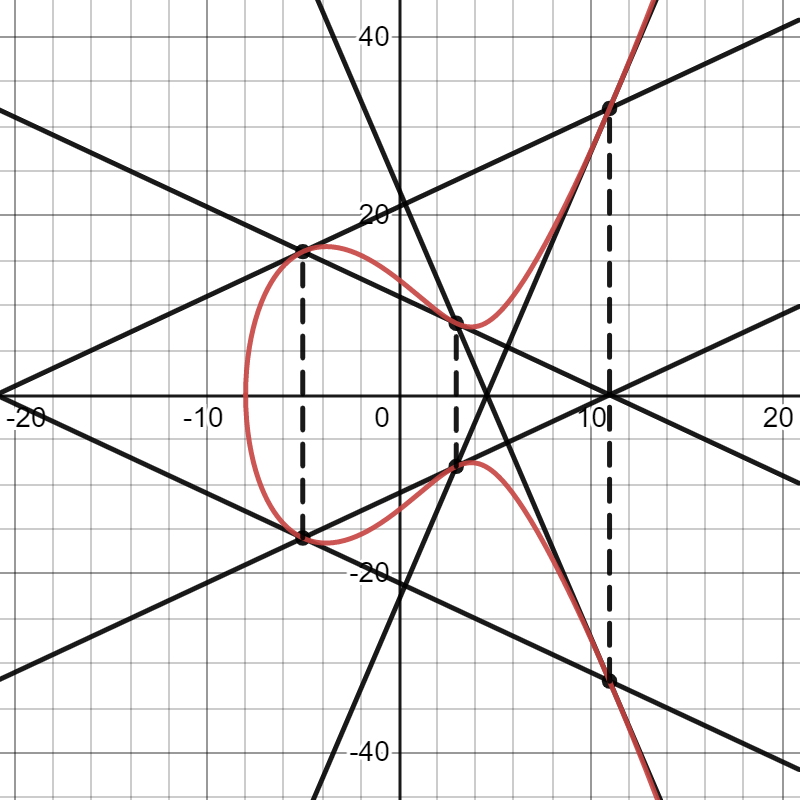
\includegraphics[width=0.5\textwidth]{desmos-graph (5).png}
\caption{\label{fig:into curve} The curve $y^2  = x^3 - 43 x + 166$ and it's points of finite order}
\end{figure}

\newpage

\bibliographystyle{agsm}
\bibliography{sample}

\end{document}